\documentclass[a4paper]{scrartcl}

\usepackage{minted}

\usepackage{tikz}
\usetikzlibrary{automata, positioning, arrows}
\tikzset{
	->, % makes the edges directed
	>=stealth', % makes the arrow heads bold
	node distance=3cm, % specifies the minimum distance between two nodes. Change if necessary.
	every state/.style={thick, fill=gray!10}, % sets the properties for each ’state’ node
	initial text=$ $, % sets the text that appears on the start arrow
}

\usepackage{amsthm, amssymb, amsmath}
\usepackage{bm}

\newtheorem{theorem}{Theorem}
\newtheorem*{theorem*}{Theorem}
\newtheorem{lemma}{Lemma}
\newtheorem*{lemma*}{Lemma}

\newtheorem{claim}{Claim}
\newtheorem*{claim*}{Claim}

\theoremstyle{definition}
\newtheorem{definition}{Definition}
\newtheorem*{definition*}{Definition}

\newcommand{\eps}{\varepsilon}
\newcommand{\card}[1]{\left\lvert #1 \right\rvert}

\title{
	Programming Languages: Lecture 7\\
	Regex
}
\author{Rishabh Dhiman}
\date{15 January 2022}

\begin{document}
\maketitle

\section{Regular Expressions Language}
\begin{itemize}
	\item Any set of strings built up from the symbols of $A$ is called a language. $A^*$ is the set of all finite strings buillt up form $A$.
	\item Each regex is a finite sequence of symbols made up of symbols from the alphabet and other symbols called operators.
	\item A regular expression may be used to describe an \emph{infinite} collection of strings.
\end{itemize}

\section{Language}
Any collection of finite strings is a language.

\section{Simple Language of Regular Expressions}
We consider a simple language of regular expressions. Assume a (finite) alphabet $A$ of symbols. Each regular expression $r$ denotes a set of strings $\mathcal L(r)$. $\mathcal L(r)$ is also called the \emph{language} spexified by the regular expression $r$.
\begin{itemize}
	\item Symbol, for $a \in A$, $\{a\}$ refers to the single element $a$.
	\item Concatenation. $\mathcal{L}(rs) = \mathcal{L}(r)\mathcal{L}(s)$.
	\item Epsilon $\eps$ denotes the language with a single element the \emph{empty} string, ``\;".
		\[L(\eps) = \{\eps\}.\]
	\item Alternation. Given two regex $r, s$; $r \mid s$ is the set of union of the languages specified by $r$ and $s$.
		\[\mathcal{L}(r \mid s) = \mathcal{L}(r) \cup \mathcal{L}(s).\]
	\item Kleene Closure $r^* = r^0 \mid r^1 \mid \cdots$ denotes an infinite union of languages.
		\[\mathcal{L}(r^*) = \bigcup_{n = 0}^{\infty} \mathcal{L}(r^n).\]
	\item $+$-closure: $r^+ = r^1 \mid r^2 \mid \cdots$.
	\item Range specifications: $[a - c] = a \mid b \mid c$.
\end{itemize}

The set of regex over an alphabet $A$ is a monoid under concatenation, also under alternation.

\section{DFA/NFA}
A regex expression can be turned into an NFA, which can be turned into a DFA.

For an NFA $N$, define $\mathcal{L}(N)$ as the set of languages that $N$ accepts.


\section{Regex to NFA Construction}
We do so by structural induction.

\begin{figure}[h]
	\centering
	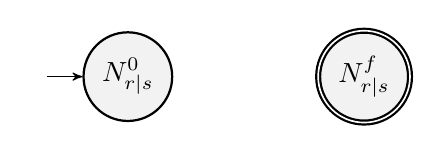
\begin{tikzpicture}
		\node[state, initial] (0) {$N_{r \mid s}^0$};
		\node[state, accepting, right of = 0] (f) {$N_{r \mid s}^f$};
	\end{tikzpicture}
	\label{Alternation}
\end{figure}

Each regex operator adds at most 2 new states and at most 4 new transitions. So, for a regex $r$, $N_r$ has at most $2 \card{r}$ and $4 \card{r}$ transitions.

\section{Extensions}
\begin{enumerate}
	\item Show how to construct a NFA for ranges and multiple ranges of symbols.
	\item Assuming $N_r$ is an NFA for the regex $r$, how will you construct NFA $N_{r^+}$.
	\item $\mathcal{L}(r\{k, n\}) = \bigcup_{k \le m \le n} \mathcal{L}(r^m)$.
	\item $\mathcal{L}(\widehat{r}) = A^* - \mathcal{L}(r)$.
\end{enumerate}
\end{document}
